\documentclass{article}
\usepackage{amsmath}
\usepackage{amsthm}
\usepackage{amssymb}
\usepackage{mathtools}
\usepackage{enumitem}
%For double angled brackets
\usepackage{MnSymbol}
\usepackage{quiver}
\usepackage[hidelinks]{hyperref}
%For bibliography
\usepackage[backend=biber]{biblatex}
%Standard theorem-like environment
\usepackage{caption}
\usepackage{graphicx}
\graphicspath{ {./images/} }

\theoremstyle{plain}
\newtheorem{thm}{Theorem}[section]

\newtheorem{prop}[thm]{Proposition}
\newtheorem{lem}[thm]{Lemma}
\newtheorem{coro}[thm]{Corollary}
\newtheorem{prob}{Problem}
\newtheorem{conj}{Conjecture}


\theoremstyle{definition}
\newtheorem{defn}[thm]{Definition}
\newtheorem{rem}[thm]{Remark}
\newtheorem{eg}[thm]{Example}
\newtheorem{egs}[thm]{Examples}
\newtheorem{fact}[thm]{Fact}
\newtheorem{task}{Task}

\DeclareMathOperator{\Hom}{Hom}
\DeclareMathOperator{\End}{End}
\DeclareMathOperator{\Aut}{Aut}
\DeclareMathOperator{\Obj}{Obj}
\DeclareMathOperator{\id}{id}
\DeclareMathOperator{\Diag}{Diag}


\addbibresource{main.bib}

\begin{document}
	\title{My Part III essay}
	\author{Hernán Ibarra Mejia}
	\maketitle
	\tableofcontents
	\section{Introduction}
	\subsection{Fundamental example}
	Take a torus and draw a directed graph on it without any edge-crossings. Label the edges of the graph too. For example, in Figure \ref{fig:k33_torus} we have drawn $K_{3,3}$, also known as the utility graph, in a torus without any crossings.
	
	\begin{figure}[h]
		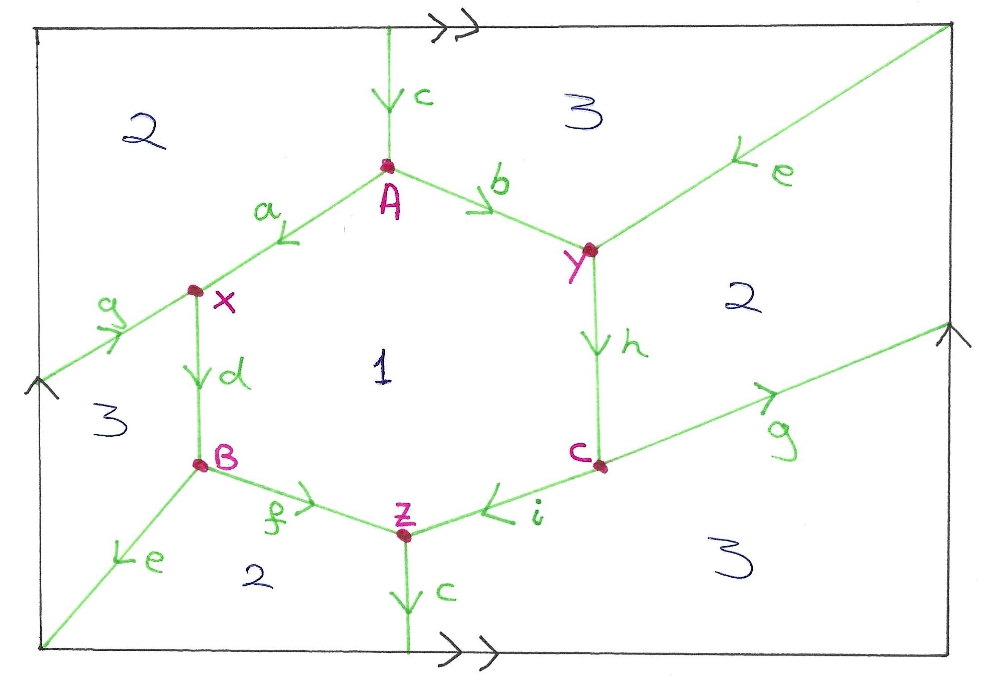
\includegraphics[scale=.5]{ut_graph_torus}
		\centering
		% https://q.uiver.app/#q=WzAsMTgsWzEsMCwiQSJdLFswLDEsIlgiXSxbMCwyLCJCIl0sWzEsMywiWiJdLFsyLDIsIkMiXSxbMiwxLCJZIl0sWzQsMSwiWSJdLFs0LDIsIkMiXSxbNSwzLCJYIl0sWzYsMiwiQSJdLFs2LDEsIloiXSxbNSwwLCJCIl0sWzksMCwiQyJdLFs4LDEsIloiXSxbOCwyLCJBIl0sWzksMywiWSJdLFsxMCwyLCJCIl0sWzEwLDEsIlgiXSxbMCwxLCJhIiwyXSxbMSwyLCJkIiwyXSxbMiwzLCJmIiwyXSxbNCwzLCJpIl0sWzUsNCwiaCJdLFswLDUsImIiXSxbMTEsNiwiZSIsMl0sWzYsNywiaCIsMl0sWzcsOCwiZyIsMl0sWzExLDEwLCJmIl0sWzEwLDksImMiXSxbOSw4LCJhIl0sWzEyLDEzLCJpIiwyXSxbMTQsMTUsImIiLDJdLFsxMywxNCwiYyIsMl0sWzE3LDE2LCJkIl0sWzEyLDE3LCJnIl0sWzE2LDE1LCJlIl1d
		\[\begin{tikzcd}[cramped,column sep=scriptsize]
			& A &&&& B &&&& C \\
			X && Y && Y && Z && Z && X \\
			B && C && C && A && A && B \\
			& Z &&&& X &&&& Y
			\arrow["a"', from=1-2, to=2-1]
			\arrow["d"', from=2-1, to=3-1]
			\arrow["f"', from=3-1, to=4-2]
			\arrow["i", from=3-3, to=4-2]
			\arrow["h", from=2-3, to=3-3]
			\arrow["b", from=1-2, to=2-3]
			\arrow["e"', from=1-6, to=2-5]
			\arrow["h"', from=2-5, to=3-5]
			\arrow["g"', from=3-5, to=4-6]
			\arrow["f", from=1-6, to=2-7]
			\arrow["c", from=2-7, to=3-7]
			\arrow["a", from=3-7, to=4-6]
			\arrow["i"', from=1-10, to=2-9]
			\arrow["b"', from=3-9, to=4-10]
			\arrow["c"', from=2-9, to=3-9]
			\arrow["d", from=2-11, to=3-11]
			\arrow["g", from=1-10, to=2-11]
			\arrow["e", from=3-11, to=4-10]
		\end{tikzcd}\]
		\caption{}
		\label{fig:k33_torus}
	\end{figure}
	
	Now consider the labels as elements of some abelian group. Each face (region) of the graph gives us a ``commutative diagram'' to which there is a corresponding equation. 
	
	For instance, face 1 in our example gives the equation
	\begin{equation}\label{eq:k33_e1}
		 fda = ihb 
	\end{equation}
	(We are taking the convention that elements are composed as functions, so we write them from right to left.) Similarly, we can write out the equations corresponding to the other faces.
	\begin{gather}
		ghe = acf \label{eq:k33_e2}\\
		bci = edg.\label{eq:k33_e3}
	\end{gather}
	Something surprising happens. These equations are \emph{interdependent}, that is, any equation is implied by all the other ones, and this holds true in all abelian groups. For instance, equation (\ref{eq:k33_e2}) implies that
	\[
		fa = c^{-1}ghe.
	\]	
	Together with equation (\ref{eq:k33_e3}) we get that
	\[
		fda = d(fa) = dc^{-1}ghe = (edg)c^{-1}h = bcic^{-1}h = ihb,
	\]
	which is exactly equation (\ref{eq:k33_e1}). What is going on?
	
	A similar game can be played on a M\"{o}bius strip and in other 2-manifolds, though we have to modify the rules when the manifold has nonempty boundary. Essentially the same interdependence phenomenon holds true, though one has to occasionally (when the manifold is non-orientable) assume that the group is not only abelian but also Boolean\footnote{Groups in which every element squares to the identity.}.
	
	These results arose in an effort to generalize the solution to a well-known problem in semigroup theory. Most of the historical remarks that follow are taken from the excellent survey by Hollings \cite{hollings2014embedding}.
	
	\subsection{Embedding monoids into groups}	
	Recall that a monoid is a set together with an associative binary operation that has an identity element, and a group is a monoid in which every element has an inverse. The problem is the following:
	
	\begin{center}
		\emph{Classify all monoids that can be embedded into a group.}
	\end{center}
		
	The question of whether a given monoid can be embedded into a group arose first in connection to ring theory. A ring can be embedded into a field if and only if it is an integral domain. In his book \emph{Moderne Algebra} \cite[Vol. I, Chap. III, Sect. 12]{van1930moderne}, van der Waerden asks for a characterization of rings which embed into skew fields, i.e. not-necessarily-commutative rings in which every non-zero element has a multiplicative inverse. Clearly rings that embed into skew fields must have no zero divisors other than zero. A ring $R$ with this latter property is called a \emph{domain}, and it follows that $R\setminus\{0\}$ is a monoid under multiplication. So, for $R$ to be embeddable into a skew-field $F$, we need $R\setminus\{0\}$ to be embed into the group $F\setminus\{0\}$.
	
	\subsection{Basic observations}
	Call a monoid \emph{embeddable} if it can be embedded into a group. Not every monoid is embeddable. To see this, consider the following definition.
	\begin{defn}[Cancellative monoids]
		Say that a monoid $M$ is \emph{left-cancellative} (respectively \emph{right-cancellative}) if $ab = ac$ (respectively $ba=ca$) implies $b = c$ for all $a,b,c\in M$. We say that a monoid is \emph{cancellative} if it is both left-cancellative and right-cancellative.
	\end{defn}
	Obviously, being cancellative is a necessary condition for being embeddable. Now, for any set $S$, consider the monoid $\End(S)$ of functions $S\to S$ under composition. Then the monoid $\End(\{0,1\})$ has two constant functions $c_0$ and $c_1$, that satisfy $c_0 c_1 = c_0 c_0$ even though $c_0\neq c_1$. Hence $\End(\{0,1\})$ is not cancellative and thus cannot be embedded into any group, and a similar result holds for $\End(S)$ whenever $|S| > 1$.
	
	In 1935, Sushkevich \cite{sushkevich1935extension} `proved' that being cancellative is equivalent to being embeddable, by explicit construction of a group out of a cancellative monoid so that the latter embeds in the former. However, Malcev quickly pointed out in a 1937 paper \cite{malcev1937immersion} that this claim could not possibly be true, since there is a cancellative monoid which does not embed into a group; Sushkevich's proof turned out to be flawed.  We now present Malcev's counterexample since it is easy to construct. First, we need another necessary condition, which Malcev called condition Z.
	
	\begin{prop}[Condition Z]
		Let $M$ be an embeddable monoid, and let $a,b,c,d,x,y,u,v\in M$. Suppose that
		\begin{align*}
			ax=by\\
			cx = dy\\
			au= bv.
		\end{align*}
		Then we must have that $cu=dv$.
	\end{prop}
	\begin{proof}
		We work in a group $G$ into which $M$ embeds. Then
		\begin{align*}
			b^{-1}a=yx^{-1}\\
			d^{-1}c = yx^{-1}\\
			b^{-1}a= vu^{-1},
		\end{align*}
		in $G$.	It follows that $d^{-1}c = vu^{-1}$ and thus $cu=dv$.
	\end{proof}
	Condition Z has a nice geometric interpretation in terms of the `interdependence diagrams' we mentioned earlier. It corresponds to a particular directed graph drawn on a sphere. In Figure \ref{fig:malc_cond_z}, we see that we are assuming that all regions commute except the upper right quadrant, which is forced to commute.
	\begin{figure}[h]
		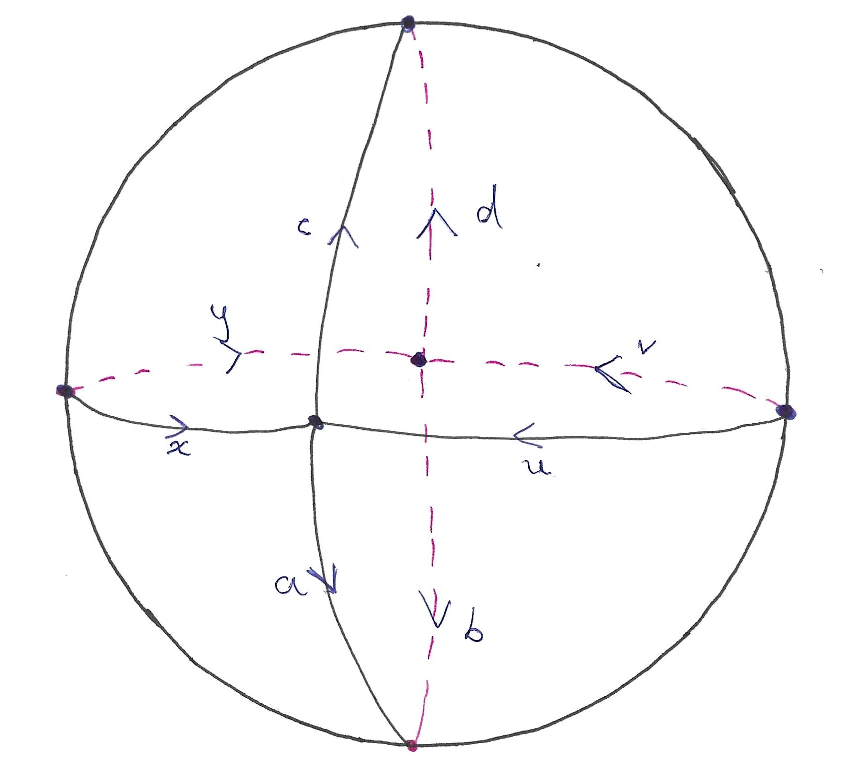
\includegraphics[scale=.35]{condition_z}
		\centering
		\caption{Malcev's condition Z as a spherical axiom}
		\label{fig:malc_cond_z}
	\end{figure}
	
	\begin{eg}[Malcev]
		Malcev constructs a monoid which is cancellative but fails to satisfy condition Z. It is natural to consider the monoid given by the presentation\footnote{In this paper, we always denote monoid presentations by square brackets, and reserve angle brackets for group presentations.}
		\[
			[\,a,b,c,d,x,y,u,v \mid ax=by,cx=dy, au= bv\,]
		\]
		And indeed, this monoid is cancellative but does not satisfy condition $Z$. Proving this rigorously requires some discussion on monoid presentations so we refer the reader to Malcev's original paper \cite{malcev1937immersion}.
	\end{eg}
	
	We remark that, if we assume commutativity, then cancellability is a sufficient condition. This is a well-known result that, while it obviously has occurred to many mathematicians since van der Waerden, is hard to find written down explicitly. The proof mimics the construction of the field of a fractions of an integral domain.
	
	\begin{prop}
		A commutative cancellative monoid is embeddable (into an abelian group).
	\end{prop}
	\begin{proof}
		Let $M$ be a commutative cancellative monoid. Define a relation on $M\times M$ by the rule $(a,b)\sim (a',b')$ if and only if $ab' = a'b$. This relation is clearly reflexive and symmetric. Transitivity holds precisely because of commutativity and cancellability: if $(a,b)\sim (a',b')$ and $(a',b')\sim (a'',b'')$ then
		\begin{equation*}
			(ab'')a' = a(a'b'')
			= a(a''b')
			= a''(ab')
			= a''(a'b)
			= (a''b)a',
		\end{equation*}
		which implies $ab'' = a''b$, i.e., $(a,b)\sim (a'',b'')$. Let $G$ be the quotient $M\times M / \sim$. 
		
		Define a binary operation on $G$ extending the operation of $M$ pointwise, that is the operation $(a,b)(c,d) = (ac,bd)$. It is easy to check that this operation respects the equivalence relation and thus is well-defined. Clearly $G$ is a group with identity $(1,1)$ and inverses defined by $(a,b)^{-1} = (b,a)$. Furthermore, $M$ embeds into $G$ via the function $m\mapsto (m,1)$ (and the group $G$ is clearly abelian).
	\end{proof}
	
	The proof also shows that there is no obvious way to replicate the construction without assuming commutativity, which is not a necessary condition. 
	
	\subsection{Other previous work and outline of the paper}
	After giving his counterexample, Malcev kept working on this problem and over the series of two more papers (\cite{malcev1939immersionI} and \cite{malcev1940immersionII}) proved the following.
	\begin{thm}[Malcev, 1940]
		There is no finite list of first-order axioms (in the language of monoids) that are necessary and collectively sufficient for a monoid to be embeddable.
	\end{thm}
	Furthermore, he explicitly gave an infinite list of conditions that were necessary and sufficient for a monoid to be embeddable. However, Malcev's conditions were complicated and the proof somewhat convoluted, so in the following years many mathematicians have extended and reinterpreted Malcev's work. Famously, Lambek \cite{lambek1951immersibility} came up with an infinite list of necessary and sufficient conditions, different from the Malcev conditions, which had a geometric interpretation in terms of polyhedra. 
	
	However, in this paper we mainly focus on the work of Krsti\'c \cite{krstic1985embedding}, to whom we attribute the idea of using the tools of geometric group theory to study the problem. We believe this approach is elegant and generalizes to other questions involving topology, which were implicitly posed by Johnstone in \cite{johnstone2008embedding}. 
	
	In the first part of this paper we give a modern account of Krsti\'c's results, and give a solution to the problem of identifying embeddable monoids. We do this by using \emph{van Kampen diagrams}, a tool often used in the area of geometric group theory. These diagrams are drawn on the plane or on the sphere (which amounts to the same thing by stereographic projection). As Lambek already pointed out, diagrams of this sort give rise to axioms necessary for a monoid to be embeddable, and all of these axioms together are sufficient. 
	
	It is natural to extend the results to other 2-manifolds, which we do in the second part of this paper. We give an original result in this direction: axioms corresponding to orientable surfaces of positive genus correspond to monoids that embed into abelian groups; and non-orientable surfaces correspond to Boolean groups. 
	\section{Krsti\'c's solution}
	\subsection{Universal Horn Axioms}
	The aim of this subsection is to prove a standard result in universal algebra, which is the first step in all searches for conditions axiomatizing embeddable monoids. First we need a definition.
	\begin{defn}[Universal Horn Axioms]
		Let $E, E_1,\ldots, E_n$ be equations in the variables $x_1,\ldots, x_m$, e.g. $x_1x_4 = x_2x_2x_5$ (we also allow the symbol $1$ to take place of a variable). A \emph{universal Horn axiom} in the \emph{language of monoids} is a propositional sentence of the form
		\[
		\forall x_1 \forall x_2 \cdots \forall x_m. (E_1\wedge E_2 \wedge \cdots \wedge E_n \implies E).
		\]		
		A universal Horn axiom in the \emph{language of groups} is defined in exactly the same way but the equations can be written in variables $\bar{x}$ or their inverses (e.g. $x_1(x_4)^{-1}x_3 = x_2$).
	\end{defn}
	\begin{rem}
		We allow for $n = 0$, so that $\forall \bar{x}. E$ is also a universal Horn axiom.
	\end{rem}
	
	For instance, the (right) cancellative law
	\[
	\forall a,b,c\,\,(ac = bc \implies a = b)
	\] 
	is a universal Horn axiom (in the language of monoids) satisfied by all groups. 
	
	From now on we use the notation $x\equiv_X y$ to mean that $x$ and $y$ are equal when considered as elements of the structure $X$. The result we need is the following and the proof below is due to Kristi\'c \cite[Section 4, Proposition 2]{krstic1985embedding}.
	\begin{lem}\label{lem:emb_iff_uha}
		A monoid $M$ is embeddable into a group if and only if whenever we have a universal Horn axiom $\varphi$ (in the language of monoids) which is satisfied by all groups, we also have $M$ satisfying $\varphi$. The same is true if we replace `group' by `abelian group' or `Boolean group' in the previous sentence.\footnote{Of course, a monoid that embeds into a Boolean group is a Boolean group.}
	\end{lem}
	\begin{proof}
		The direction $(\Rightarrow)$ is trivial. Indeed, universal Horn axioms are clearly preserved under submonoids. In other words, if $N$ satisfies a universal Horn axiom $\varphi$ and $M$ is a submonoid of $N$, then $M$ satisfies $\varphi$.  
		
		Conversely $(\Leftarrow)$ is trivial for abelian and for Boolean groups. This is because
		\[
			\forall a,b. (ab=ba) \,\,\,\text{ and }\,\,\, \forall x. (x^2 = 1),
		\]
		and the cancellative law are universal Horn axioms. But if a monoid satisfies $\forall x. (x^2 = 1)$ then it is already a Boolean group. In addition, if a monoid is commutative and cancellative we showed in the introduction that it embeds into an abelian group.
		
		It remains to show $(\Leftarrow)$ for general groups. Suppose $M$ is a monoid which satisfies all universal Horn axioms satisfied by all groups; we need to show that $M$ is embeddable.
		
		We give a presentation for the monoid, say $M = [A\mid R]$ where
		\[
			R = \{\, w_i = w_i' \,\mid\, i \in I\,\}
		\]
		for some set $I$. Consider the group $G \coloneqq \langle A\mid R\rangle$ with the same presentation. By a suitable universal property, there is a unique homomorphism $M \to G$ preserving the generators. We show that this homomorphism is injective.
		
		Let $w,w'$ be two words in the alphabet $A$; we need to prove that $w\equiv_G w'$ implies $w\equiv_M w'$. Let $F\coloneqq F(A)$ be the free group generated by $A$. Define $W \coloneqq w(w')^{-1}$ and $W_i \coloneqq w_i(w_i')^{-1}$ for $i\in I$ considered as elements of $F$.
		
		If $w\equiv_G w'$ then $W \equiv_G 1$. Hence $W$, as an element of $F$, belongs to the normal subgroup of $F$ generated by the $W_i$'s. It follows that
		\begin{equation}\label{eq:word_norm_cl}
			W \equiv_F \prod_{j = 1}^{k}h_j \,(W_{i_j})^{\epsilon_j}\, h_j^{-1}
		\end{equation}
		for some indices $i_1,\ldots, i_k$, some $h_j\in F$, and some $\epsilon_j= \pm 1$. 
		
		Consider the alphabet $A$ as a set of variables and let $\bar{a}$ be all variables appearing in (\ref{eq:word_norm_cl}). Then the expression (\ref{eq:word_norm_cl}) implies that in any group we have
		\[
			\forall \bar{a}. \,\,(W_{i_1} = 1 \wedge \cdots \wedge W_{i_k} = 1 \implies W = 1),
		\]
		or, equivalently,
		\[
			\forall \bar{a}. \,\,(w_{i_1} = w_{i_1}' \wedge \cdots \wedge w_{i_k} = w_{i_k}' \implies w = w').
		\]
		This is a universal Horn axiom so, by assumption, $M$ satisfies this axiom and thus $w\equiv_M w'$ as desired.
	\end{proof}
	The following remark is for general interest and not used in the rest of the paper.
	\begin{rem}
		The group $G$ employed in the proof is called the \emph{universal enveloping group} of the monoid $M$ and does not depend (up to isomorphism) on the presentation used for $M$. It is the left adjoint to the forgetful functor from groups to monoids (whose existence follows from the general adjoint functor theorem). This implies that if $M$ embeds into \emph{any} group then it embeds into its universal enveloping group.
	\end{rem}
	
	\subsection{Diagrams}
	We need a definition from geometric group theory, that of a van Kampen diagram. The definition below is slightly different than the standard one, and is better suited to our purposes. From now on, we fix some countable set $V$ of variable symbols. 
	
	Let $\Sigma$ be a connected closed surface. A $\Sigma$\emph{-diagram} is a cellular decomposition $D$ of $\Sigma$ such that each edge (1-cell) of $D$ is labelled with a variable $x\in V$ and an arrow giving its orientation. We also allow for labelling an edge with the symbol $1$ instead of a variable.
	
	A $\Sigma$-diagram $D$ is said to be \emph{monoidal} if the boundary of each region (2-cell) of $D$ is of the form shown in Figure \ref{fig:monoidal_bndy}.
	
	\begin{figure}[h]
		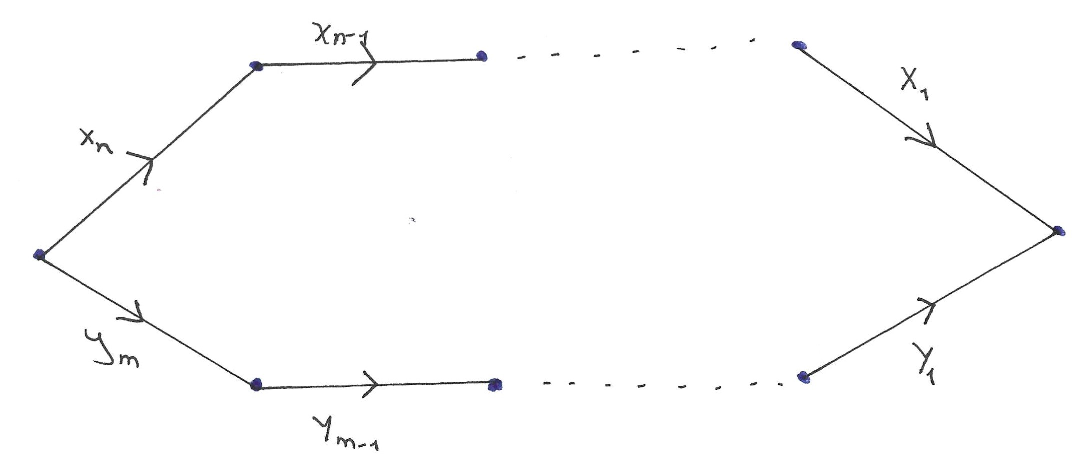
\includegraphics[scale=.5]{monoidal_face}
		\centering
		\caption{Monoidal boundary}
		\label{fig:monoidal_bndy}
	\end{figure}
	
	Let $r$ be a 2-cell of a $\Sigma$ diagram $D$. The boundary of $r$ can be associated with an equation in the language of groups, saying that the boundary word is trivial. Formally, we pick a vertex in the boundary of $r$ and start reading the labels in some direction (either clockwise or counter-clockwise) until we end back at the starting vertex. We write an expression from right to left as follows. If the arrow label of the edge agrees with the direction we are taking we write that variable, whereas if it disagrees we write the formal inverse of that variable. This process yields a product of variables and inverses of variables, say $x_1^{\epsilon_1}\cdots x_n^{\epsilon_n}$ where $x_i\in V$ and $\epsilon_i=\pm 1$ for all $i$. We define the $r$\emph{-equation}, denoted $E_r$, to be 
	
	\[
		x_1^{\epsilon_1}\cdots x_n^{\epsilon_n} = 1.
	\]
	
	Of course, we made some arbitrary choices when defining $E_r$, but these are immaterial since different choices result in equivalent equations over any group. Indeed, if $E_r$ is $w = 1$ for some word (term) $w$, then choosing a different direction of the boundary yields the equation $w^{-1} = 1$, whilst choosing a different starting vertex yields (possibly after introducing some cancelling pairs $xx^{-1}$ or $x^{-1}x$) the equation $twt^{-1} = 1$ for some word $t$; and all these equations are equivalent in all groups. So, technically, $E_r$ is only defined up to equivalence of equations over the theory of groups, but we will often abuse language and talk about `the' $r$-equation. For instance, if $xy^2 = 1$ is the $r$-equation then so is $yxy = 1$ and even $y^2 = x^{-1}$.
	
	For $D$ a $\Sigma$-diagram and $r$ a $2$-cell of $D$, we define the $(D,r)$\emph{-axiom} to be the universal Horn axiom (in the language of groups)
	\[
		\forall \bar{x}. \left(\,\,\,\, \bigwedge_{\mathclap{\substack{s\in D^{(2)}\\
					s\neq r}}} E_s \implies  E_r \,\,\right).
	\]
	As before, the $(D,r)$\emph{-axiom} is only defined up to equivalence over groups.
	
	For a given $D$ we refer to the collection of all $(D,r)$-axioms, for $r$ a 2-cell of $D$, simply as the $D$-axioms. Now we define the $\Sigma$\emph{-axioms} to be all $D$-axioms for $D$ a $\Sigma$-diagram. Then the collection of all $\Sigma$-axioms is a theory in the language of groups. 
	
	We would like to now restrict these axioms to those that make sense in an arbitrary monoid. If the diagram $D$ is monoidal, then any $r$-equation can be uniquely written as
	\[
		x_1x_2\cdots x_n = y_1 y_2\cdots y_m,
	\]
	which is a generic equation in the language of monoids. Thus the $(D,r)$-axiom is just an axiom in the language of monoids. When we are working with monoids, the $\Sigma$-axioms refer to all $D$-axioms for $D$ a monoidal $\Sigma$-diagram. Context usually makes it clear to which $\Sigma$-axioms we are referring to, but, if necessary to differentiate them, we will talk about the $\Sigma$ group axioms and the $\Sigma$ monoid axioms.	
	
	In this section we will study the case of the 2-sphere $\Sigma = \mathbb{S}^2$, and we refer in this case to \emph{spherical diagrams}, and to the resulting axioms as the \emph{spherical axioms}.
	
	\begin{eg}\label{eg:sph_canc}
		We have seen in the introduction that Malcev's condition Z is a spherical monoid axiom. The left-cancellative law is also a spherical monoid axiom as we see in Figure \ref{fig:sph_canc}.
		
		\begin{figure}[h]
			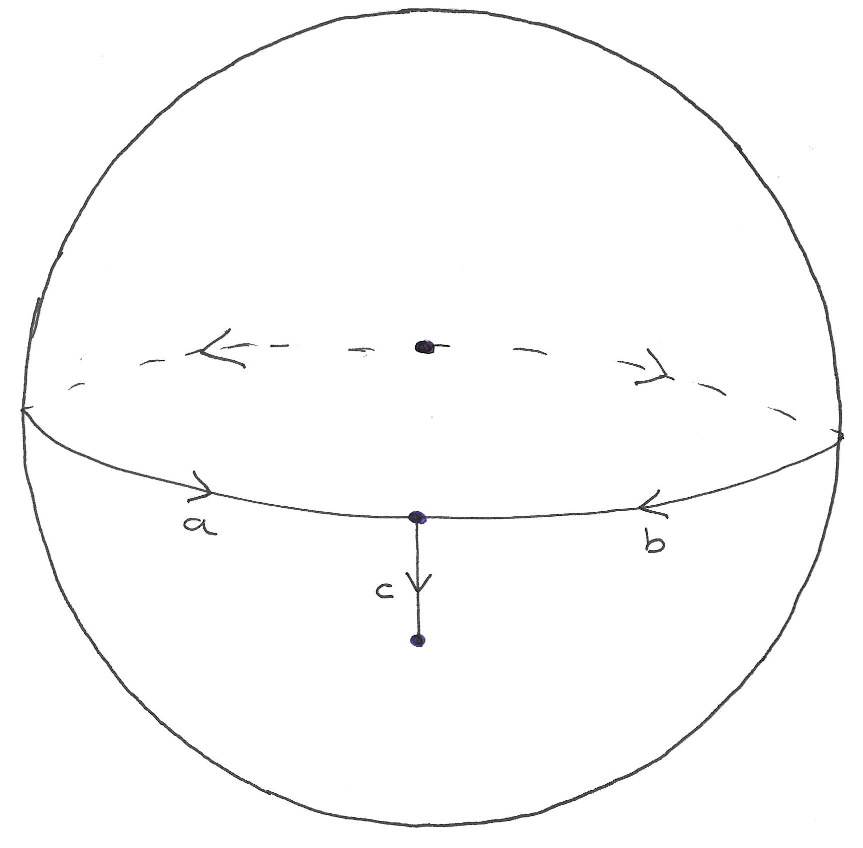
\includegraphics[scale=.35]{canc_law_sph}
			\centering
			\caption{Cancellation law as a spherical axiom}
			\label{fig:sph_canc}
		\end{figure}
		
		(This also shows why we do not restrict to \emph{regular} cell complexes.) We can get the right-cancellative law by reversing the arrows.
	\end{eg}
	\begin{rem}\label{rem:single_face_diag}
		A word on single-faced diagrams. If a diagram $D$ has only one 2-cell $r$ then the $(D,r)$-axiom takes the form $\forall \bar{x}. E$, which is the degenerate case in our definition of Horn axioms. On the sphere, single-faced diagrams are more-or-less trivial. For example, a monoidal diagram with only one region might have a boundary which is a single line of 1-cells. The resulting axiom will read something like
		\[
			\forall \bar{x}. x_1\ldots x_n = x_1 \ldots x_n
		\] 
		which is not interesting. However, single-faced diagrams will become relevant on other surfaces so it is important to include them in the definition.
	\end{rem}
	\subsection{Embeddability and the spherical axioms}
	In this subsection we prove that a monoid is embeddable if and only if it satisfies the spherical monoid axioms. The geometric group theorist will recognize that the proofs in this subsection are essentially taken from the proof of \emph{van Kampen's lemma}, a classical result in geometric group theory due to van Kampen \cite{vankampen1933lemma}. This result was known to Krsti\'c, who cites van Kampen in \cite{krstic1985embedding}.
	
	We first point out that groups satisfy the spherical axioms. This is not hard to see intuitively (recall Malcev's condition Z). We give a proof using some topology and the fundamental group.
	\begin{prop}\label{prop:grp_sph}
		Groups satisfy the spherical axioms.
	\end{prop}
	\begin{proof}
		Let $D$ be a spherical diagram on variables $\bar{x} \coloneqq (x_1,\ldots,x_n)$, and $r$ a 2-cell of $D$. Suppose the $(D,r)$-axiom takes the form
		\[
			\forall \bar{x}. \left(w_1 = 1 \wedge \cdots \wedge w_m = 1 \implies w = 1\right)		
		\]
		for words $w,w_1,\ldots, w_m$ in the variables $\bar{x}$ (or their inverses).
		
		Let $G$ be the group given by the presentation
		\[
			\langle x_1,\ldots, x_n \mid w_1,\ldots, w_m\rangle
		\]
		It suffices to prove that $w\equiv_G 1$. This is because if there is any group $H$ and elements $\bar{h} = (h_1,\ldots, h_n)\in H^n$ satisfying $w_i(\bar{h}) = 1$ then, by a suitable universal property, there would be a unique homomorphism $\varphi \colon G \to H$ sending $x_i \mapsto h_i$, and thus $w(\bar{h}) = \varphi(w) = \varphi(1) = 1$ as desired. Then $H$ satisfies the $(D,r)$-axiom, and since $H$, $D$, and $r$ were arbitrary the result follows.
		
		Now we build a topological space $P$, called the \emph{presentation complex} of $G$. We take a wedge of circles $n$ circles, one for each variable, and we give them an orientation. Afterwards, we attach $m$ discs (2-cells) by gluing their boundaries to the loops corresponding to the words $w_i$ (this is where we use the oriented labels). Then $P$ is path-connected and the Seifert-Van Kampen theorem implies that $\pi_1(P) = G$.
		
		Let $D'$ be the subcomplex of $D$ obtained by taking out $r$ but keeping its boundary. We construct a map $D' \to P$ as follows. Every vertex of $D'$ can be mapped to the unique vertex of $P$. Every edge of $D'$ maps to the corresponding circle in $P$ given by the labels. Every region of $D'$ maps to the corresponding disc attached to $P$, again this is given by the labels on the boundaries. This is a finite collection of maps from closed subspaces of $D'$ to $P$ which agree on overlaps and their domains cover all of $D'$. By the gluing lemma this defines a unique continuous map $D' \to P$.
		
		There is also a continuous map $S^1\to D'$ mapping to the boundary of $r$, and a continuous map $S^1\to P$ to the loop spelling out $w$. Furthermore the diagram
		% https://q.uiver.app/#q=WzAsMyxbMCwwLCJTXjEiXSxbMiwwLCJEJyJdLFsxLDEsIlAiXSxbMCwxXSxbMCwyXSxbMSwyXV0=
		\[\begin{tikzcd}
			{S^1} && {D'} \\
			& P
			\arrow[from=1-1, to=1-3]
			\arrow[from=1-1, to=2-2]
			\arrow[from=1-3, to=2-2]
		\end{tikzcd}\]
		commutes. All of these spaces are path-connected. By functoriality of $\pi_1$, we see that the induced diagram 
		% https://q.uiver.app/#q=WzAsMyxbMCwwLCJcXG1hdGhiYntafSJdLFsyLDAsIjEiXSxbMSwxLCJcXHBpXzEoUCk9RyJdLFswLDFdLFswLDJdLFsxLDJdXQ==
		\[\begin{tikzcd}
			{\mathbb{Z}} && 1 \\
			& {G}
			\arrow[from=1-1, to=1-3]
			\arrow[from=1-1, to=2-2]
			\arrow[from=1-3, to=2-2]
		\end{tikzcd}\]
		commutes. Hence we see that the map $\mathbb{Z} \to G$ is trivial (here we crucially use the fact that $D$ is homeomorphic to $\mathbb{S}^2$, for then $D'$ is contractible). But this maps sends $1 \mapsto w$, hence $w$ is trivial, as desired.
	\end{proof}
	Recall that a word in a free group is said to be \emph{reduced} if no cancelling pairs $xx^{-1}$ and $x^{-1}x$ occur as subwords. A word is said to be \emph{cyclically reduced} if any cyclic permutation of the word gives a reduced word. For example, $xywzw^{-1}x^{-1}$ is reduced but not cyclically reduced since $x^{-1}xywzw^{-1}$ is a cyclic permutation of the word. Removing the $x$'s gives a cyclically reduced word $ywzw^{-1}$.
	\begin{thm}\label{thm:emb_iff_sph}
		A monoid is embeddable if and only if it satisfies the spherical (monoid) axioms.
	\end{thm}
	\begin{proof}
		By the previous proposition, groups satisfy the spherical group axioms. In particular, they satisfy the spherical monoid axioms. As these are universal Horn axioms, it follows from Lemma \ref{lem:emb_iff_uha} that embeddable monoids satisfy the spherical monoid axioms.
		
		Conversely, assume that a monoid $M$ satisfies the spherical axioms. Again by Lemma \ref{lem:emb_iff_uha}, it suffices to show that if $\bar{x} = (x_1,\ldots, x_n)$ and
		\[
			\Phi\coloneqq \forall\bar{x}. \left(w_1 = w_1' \wedge \cdots \wedge w_m = w_m' \implies  w = w'\right) 
		\]		
		is a universal Horn axiom satisfied by all groups then $M$ satisfies $\Phi$. Here we are working in the language of monoids so all $w$'s are in the variables $\bar{x}$ but not their inverses. To work with groups, we also define $W \coloneqq w(w')^{-1}$ and $W_i \coloneqq w_i(w_i')^{-1}$ for all $i$. 
		
		We can assume that $W$ is a cyclically reduced word. Indeed, $M$ is cancellative by Example \ref{eg:sph_canc}, so after applying right-cancellativity to $w = w'$ we would get rid of cancelling pairs in $W$, making $W$ reduced. Similarly, by applying left-cancellativity, we get rid of any cancelling pairs that would arise after a cyclic permutation.
		
		As in the proof of the previous proposition, we consider the ``most general group in which $\Phi$ can fail'', namely
		\[
			G\coloneqq \langle x_1,\ldots,x_n \mid W_1,\ldots, W_m\rangle.
		\]
		We know that $\Phi$ holds in all groups so in particular it holds in $G$, hence $W \equiv_G 1$. By definition of a presentation, this means that if $F \coloneqq F(\bar{x})$ is the free group with generators $\bar{x}$ then $W$ belongs to the normal subgroup of $F$ generated by $W_1,\ldots, W_n$. In particular,
		\[
			W \equiv_F \prod_{j = 1}^{k}h_j \,(W_{i_j})^{\epsilon_j}\, h_j^{-1}
		\]
		for some indices $i_1,\ldots, i_k$, some $h_j\in F$, and some $\epsilon_j= \pm 1$. We construct a two-dimensional cell complex with $k$ 2-cells (commonly referred to as a ``lollipop diagram'') as in Figure \ref{fig:lollipop_diagram}. 
		
		\begin{figure}[h]
			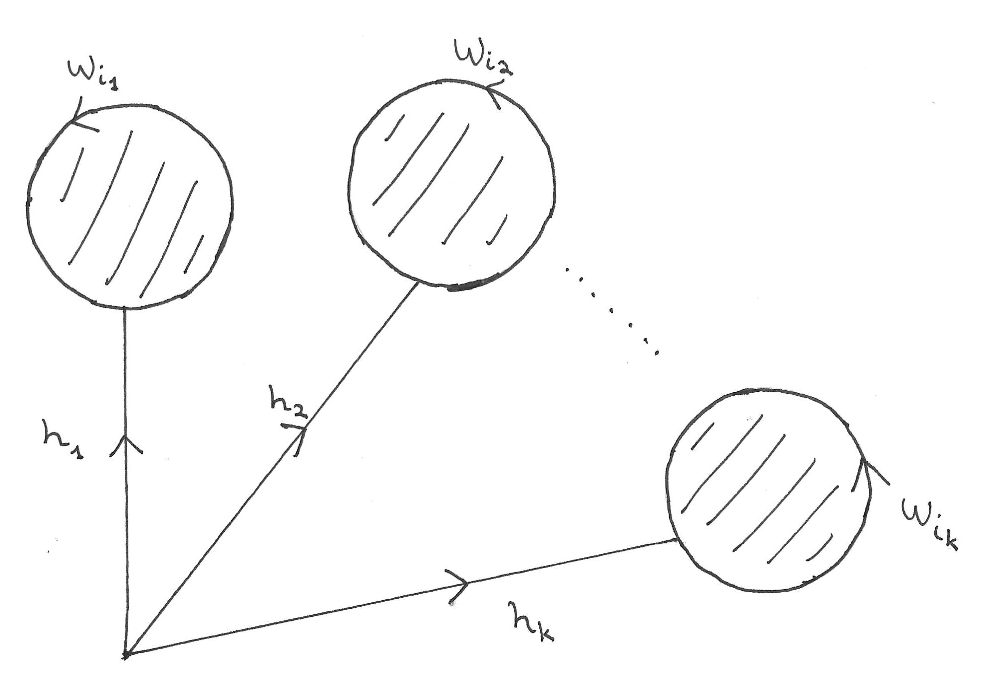
\includegraphics[scale=.5]{lollipop_diagram}
			\centering
			\caption{Lollipop diagram}
			\label{fig:lollipop_diagram}
		\end{figure}		
		
		We would like to attach a 2-cell to the outside boundary of this complex to make it a spherical diagram. Then $M$ will satisfy this spherical diagram, which means that $M$ satisfies $\Phi$ as a result. Unfortunately this does not work because the outside boundary is not the word $W$, it is only $W$ in the group $F$. In fact, the resulting spherical diagram is not monoidal in general (the boundary of the new 2-cell has the wrong form), so our assumption on $M$ does not apply.
		
		However, the fact that the boundary word is $W$ in $F$, and since $W$ is reduced, means that it will be exactly equal to $W$ after some elementary reductions, i.e. by eliminating cancelling pairs $xx^{-1}$ and $x^{-1}x$. We can mimic this elimination procedure by modifying the cell complex.
		
		Let $e,e'$ be two consecutive edges of the outside boundary (we are taking a direction for this boundary and we assume $e$ comes before $e'$) that are labelled with the same variable but go in opposite orientation. If the final vertex of $e'$ coincides with the initial vertex of $e$ then $e,e'$ is a loop, and we can delete it, together with everything it may enclose, see Figure \ref{fig:lolli_del}.
		
		\begin{figure}[h]
			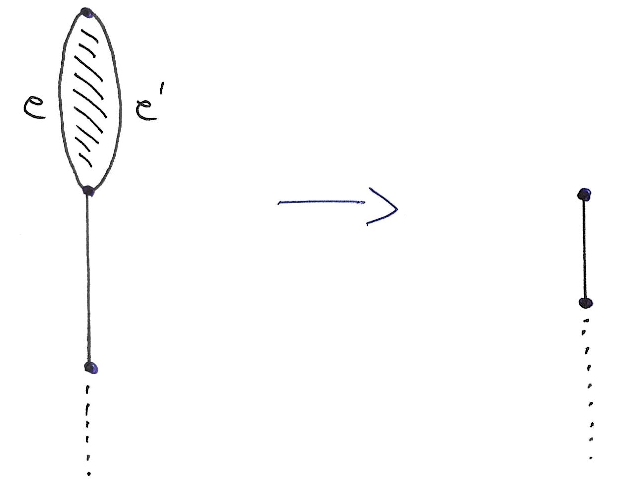
\includegraphics[scale=.5]{del_canc_van_kamp}
			\centering
			\caption{}
			\label{fig:lolli_del}
		\end{figure}		
		
		Otherwise we can fold $e$ and $e'$ onto each other, the only restriction being that we label the resulting edge in the direction of $e$ and, if these two edges happen to be on the boundary of the same 2-cell, we need to fold them `inside' as in Figure \ref{fig:lolli_fold}.
		
		\begin{figure}[h]
			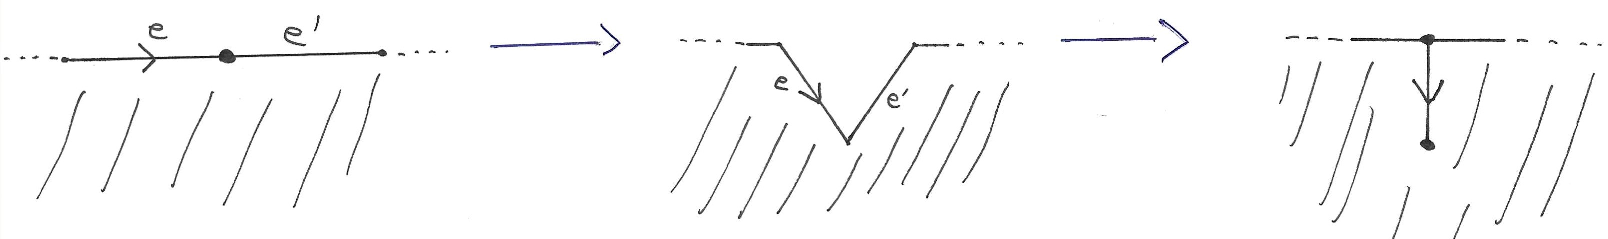
\includegraphics[scale=.4]{fold_van_kamp}
			\centering
			\caption{}
			\label{fig:lolli_fold}
		\end{figure}
		
		This process decreases the number of 1-cells and leaves the labels of the boundary of the 2-cells unchanged (it might delete some trivial 2-cells but that is okay). By repeating these steps we arrive at a new cell complex whose 2-cells have as boundaries some $W_i$ and the outside boundary is just $W$ (here we use the fact that $W$ is cyclically reduced rather than just reduced). Attach a $2$-cell to the outside boundary and we are done.
	\end{proof}
	This gives a hint of the aforementioned Malcev's theorem, which says that the class of all embeddable monoids admits no finite first-order axiomatization. As there are infinitely many spherical diagrams, there are infinitely many spherical axioms and there is no a priori reason why these reduce to a finite list of axioms.
	\section{Non-spherical surfaces}
	\subsection{Statement of the result}
	We denote by $\mathbb{T}_n$ the connected sum of $n$ copies of the torus $\mathbb{T}^2$, and similarly we write $\mathbb{P}_n$ for the connected sum of $n$ copies of the projective plane $\mathbb{P}^2$. Theorem \ref{thm:emb_iff_sph} admits the following generalization.
	\begin{thm}\label{thm:emb_surf_class}
		Let $M$ be a monoid and $n>0$ an integer.
		\begin{enumerate}[label=\textnormal{(}\alph*\textnormal{)}]
			\item $M$ is embeddable into a group iff it satisfies the spherical axioms.
			\item $M$ is embeddable into an abelian group iff it satisfies the $\mathbb{T}_n$-axioms.
			\item $M$ is a Boolean group iff it satisfies the $\mathbb{P}_n$-axioms.
		\end{enumerate}
	\end{thm}
	\begin{rem}\label{ref:emb_surf_class}
		We can immediately prove parts of the theorem with the knowledge we have so far. Obviously (a) is just Theorem \ref{thm:emb_iff_sph}. 
		
		The ($\Leftarrow$) direction of (b) and (c) are easy to see. We know that $M$ is embeddable into an abelian group iff it is commutative and cancellative. Assume that $M$ satisfies the $\mathbb{T}_n$-axioms. Then we can draw $\mathbb{T}_n$-diagram so that we get commutativity as a result of one of the associated axioms.	When $n=1$ it will be a single-faced diagram that gives us the axiom $\forall a,b. ab = ba$, see Remark \ref{rem:single_face_diag}. If $n=2$ the diagram of Figure \ref{fig:comm_t_2} clearly works.
		
		\begin{figure}[h]
			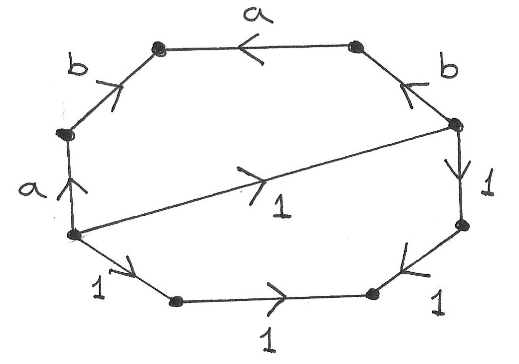
\includegraphics[scale=.5]{t_2_comm}
			\centering
			\caption{}
			\label{fig:comm_t_2}
		\end{figure}

	 	For general $n$ we can extend Figure \ref{fig:comm_t_2} in an obvious way. See Figure \ref{fig:comm_t_5} for the case $n=5$, where $[x,y]$ denotes the commutator of $x$ and $y$.
	 	
	 	\begin{figure}[h]
	 		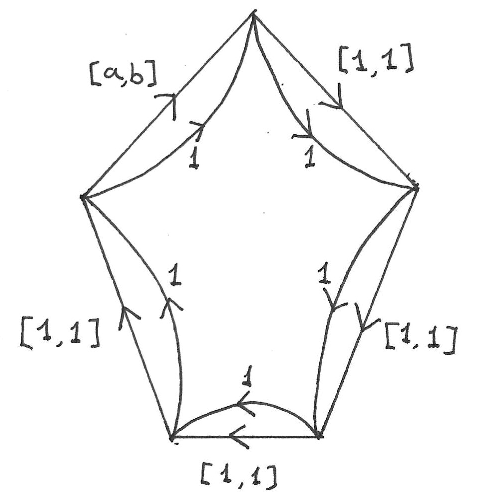
\includegraphics[scale=.5]{t_5_comm}
	 		\centering
	 		\caption{}
	 		\label{fig:comm_t_5}
	 	\end{figure}
		
		The cancellative law is also implied by a diagram; we only need to prove left-cancellativity since we already have that $M$ is commutative. For $n=1$ consider the diagram of Figure \ref{fig:canc_t_1}
		
		\begin{figure}[h]
			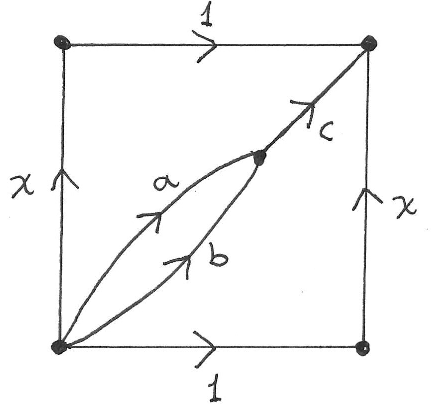
\includegraphics[scale=.5]{torus_canc}
			\centering
			\caption{}
			\label{fig:canc_t_1}
		\end{figure}
		
		This gives the axiom 
		\[
			\forall x,a,b,c.\, (ca = x \wedge cb = x \implies a = b)
		\]
		which obviously implies left-cancellativity. As before, this diagram generalizes to general $n$ by ``padding with 1s''.
		
		For Boolean groups the situation is even simpler since we only have to prove that if $M$ satisfies the $\mathbb{P}_n$-axioms then $M$ satisfies $\forall a. (a^2 = 1)$. The relevant diagram is evident, see Figure \ref{fig:bool_p_2} for the case $n=2$.
		
		\begin{figure}[h]
			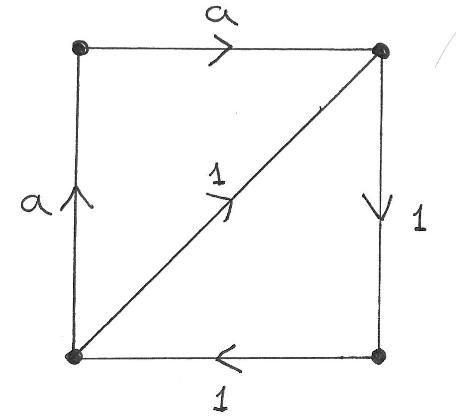
\includegraphics[scale=.5]{p_2_bool}
			\centering
			\caption{}
			\label{fig:bool_p_2}
		\end{figure}
		
		Thus the only nontrivial parts of the theorem are the direction $(\Rightarrow)$ of (b) and (c). We need some facts about diagrams before tackling the rest of the proof.
	\end{rem}
	\subsection{Implications between diagrams}
	Let $D,D'$ be $\Sigma$-diagrams with $r\in D^{(2)}$ and $r'\in D'^{(2)}$. We write 
	\[
		(D',r') \vdash (D,r)
	\]
	to indicate that the $(D',r')$-axiom implies the $(D,r)$-axiom in any given group. Further, we write $(D'\vdash D)$ if for all $r\in D^{(2)}$ there is some $r'\in D'^{(2)}$ such that $(D',r') \vdash (D,r)$. In particular, if $(D'\vdash D)$ then the $D'$-axioms imply the $D$-axioms.
	
	Recall that a \emph{subdivision} of an edge is to replace it with two new edges with a vertex in the middle. In the context of diagrams, we agree that a subdivision preserves the orientation of the arrows and adds a \emph{fresh variable}, i.e. a variable which does not appear in the rest of the diagram (this last point is important), see Figure \ref{fig:subdivision}.
	
	\begin{figure}[h]
		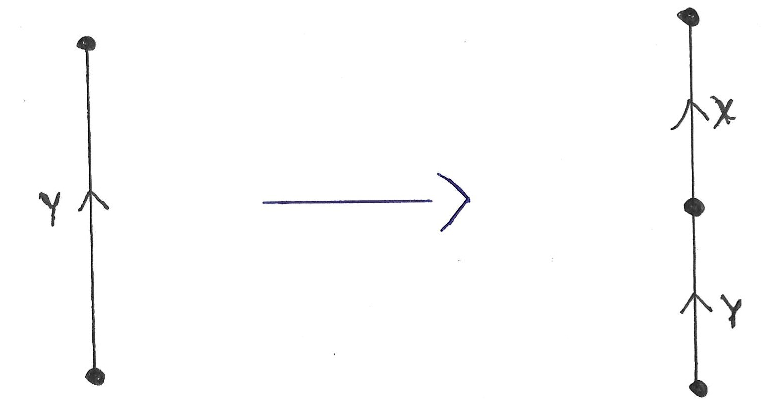
\includegraphics[scale=.5]{subdivision}
		\centering
		\caption{}
		\label{fig:subdivision}
	\end{figure} 
	
	If $D$ is a $\Sigma$-diagram and $D'$ is obtained by repeated subdivision of the edges of $D$ we call $D'$ an \emph{expansion} of $D$.
	\begin{lem}
		If $D$ is a $\Sigma$-diagram and $D'$ is an expansion of $D$, then $(D'\vdash D)$.
	\end{lem}
	\begin{proof}
		As the $\vdash$ relation is transitive, we can assume that $D'$ is the result of subdividing a single edge of $D$. Then the $D'$-axioms are just the $D$-axioms but some words will contain a fresh variable, say $x$, or its inverse, somewhere. We can just set $x = 1$ to recover the $D$-axioms (here we use the fact that $x$ is not used as a label in $D$).
	\end{proof}
	
	We can also add edges to the the diagram $D$ in two other ways. First, we can add a new edge connecting two vertices that bound the same region, effectively replacing the region by two regions, see Figure \ref{fig:div_face}. We only insist that the added edge is labelled by a fresh variable, but make no restrictions on the direction of the edge.
	
	\begin{figure}[h]
		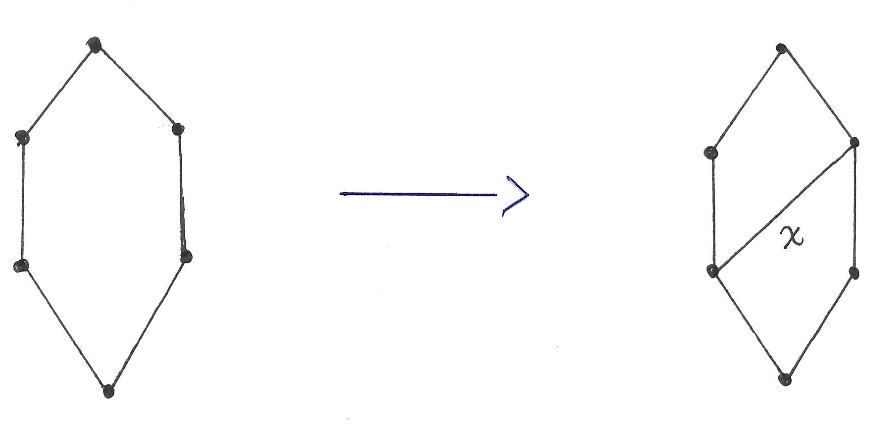
\includegraphics[scale=.5]{split_face}
		\centering
		\caption{}
		\label{fig:div_face}
	\end{figure} 
	
	The other way to add edges is by adding a vertex to the interior of a region and connecting it to a vertex in the boundary, see . Again, the new edge has to be labelled by a fresh variable.
	
	\begin{figure}[h]
		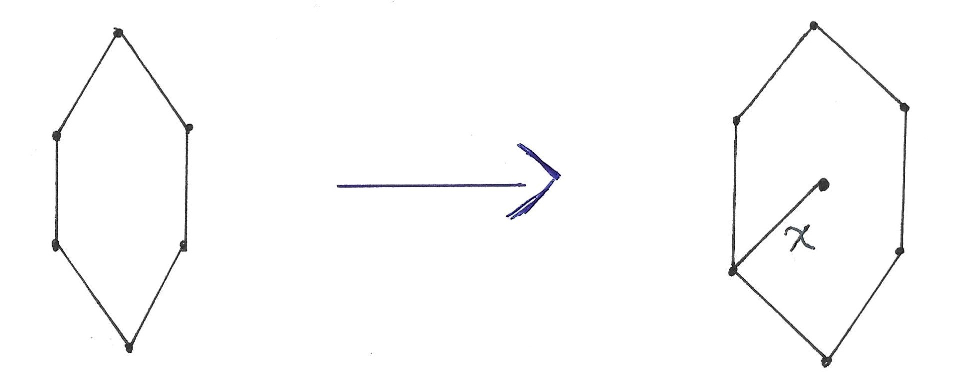
\includegraphics[scale=.5]{add_edge}
		\centering
		\caption{}
		\label{fig:new_edge_and_vertex}
	\end{figure}
	
	If $D'$ is a diagram obtained by repeatedly adding edges as above we say that $D'$ is a \emph{superdiagram} of $D$ or, equivalently, that $D$ is a \emph{subdiagram} of $D'$.
	
	\begin{lem}
		If $D$ is a $\Sigma$-diagram and $D'$ is a superdiagram of $D$, then $(D'\vdash D)$.
	\end{lem}
	\begin{proof}
		As before, we can assume that $D'$ is obtained from $D$ by adding a single edge. If this edge is added by not dividing the region as in Figure \ref{fig:new_edge_and_vertex} then it is obvious that the equation obtained is equivalent to the one obtained from the original diagram (we just added a cancelling pair).
		
		\begin{figure}[h]
			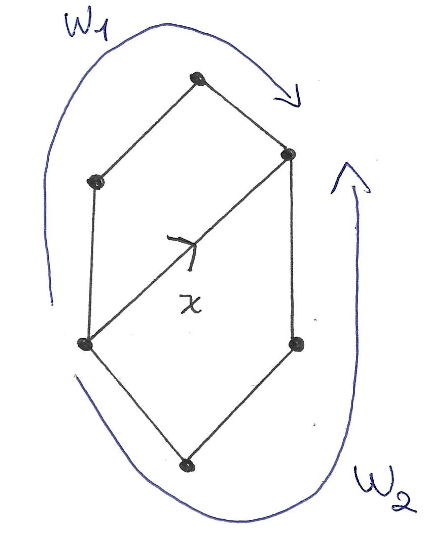
\includegraphics[scale=.5]{split_face_label}
			\centering
			\caption{}
			\label{fig:div_face_2}
		\end{figure}
		
		If the edge is added as in Figure \ref{fig:div_face_2} then, instead of taking $x=1$ as is our usual strategy, we take $x = w_1$. Then we see that the $D'$-equations are just the $D$-equations but with $w_1 = w_1$ added, so the interdependence of the $D'$-equations implies that of the $D$-equations.
	\end{proof}
	\subsection{Proof of the result}
	The key lemma is the following.
	\begin{lem}\label{lem:main_lem}
		Abelian groups satisfy the $\mathbb{T}_n$-axioms, and Boolean groups satisfy the $\mathbb{P}_n$ axioms.
	\end{lem}
	\begin{proof}
		We prove that abelian groups satisfy the $\mathbb{T}_1$-axioms since the general result is proven in essentially the same way as in this special case. Consider a $\mathbb{T}_1$-diagram $D$ drawn on the standard square with sides identified. We will modify this diagram such that the boundary of the square consists of edges and vertices (in contrast, this is not true for the $\mathbb{T}_1$-diagram in the introduction).
		
		Firstly, we subdivide edges at the points where they enter or exit the boundary of the square. Secondly, if there is no vertex where the four corners of the square get identified, we add a vertex and connect it to any vertex that bounds the region containing that corner. Thirdly, if going around the boundary of the square we find two consecutive vertices which are not connected by an edge, we add the missing edge. 
		
		We can do this using the rules described in the previous subsection to obtain $D'$, a superdiagram of an expansion of $D$. By the results of the previous subsection, $(D' \vdash D)$; hence it is enough to work with $D'$.
		
		Now we `forget' that the square has its sides identified and just regard it as a square on the plane, say. The diagram is now a cellular decomposition of the square and by adding a 2-cell to the boundary of the square we get a spherical diagram, say $D''$.
		
		\begin{figure}[h]
			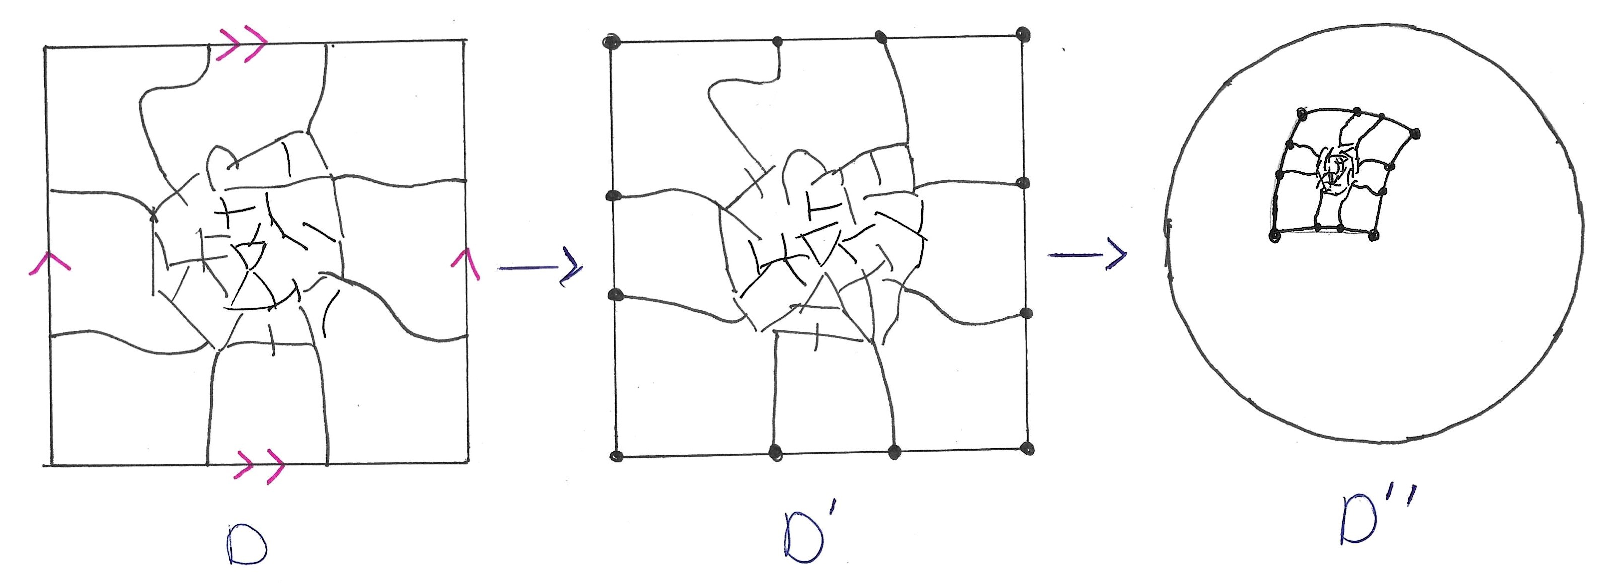
\includegraphics[scale=.45]{sq_to_sph}
			\centering
			\caption{Proof of Lemma \ref{lem:main_lem}}
			\label{fig:proof_main_lem}
		\end{figure}
		
		This spherical diagram has the same associated equations as the $\mathbb{T}_1$-diagram but it has one more equation of the form $ww'=w'w$ for words $w,w'$. This equation is valid in all abelian groups so it follows that for abelian groups the $D''$-axioms imply the $D'$ axioms and hence the $D$-axioms. 
		
		For non-spherical surfaces other than $\mathbb{T}_1$ the same proof works by use of the standard polygons with sides identified. In the case of $\mathbb{T}_n$ the boundary of the polygon will give an equation of the form
		\[
			[w_1,w_1'][w_2,w_2']\cdots[w_n,w_n'] = 1,
		\]
		which is valid in all abelian groups. For $\mathbb{P}_n$ the equation will be of the form
		\[
			w_1^2w_2^2\cdots w_n^2 = 1,
		\]
		 which is valid in all Boolean groups.
	\end{proof}
	\begin{proof}[Proof of Theorem \ref{thm:emb_surf_class}]
		We have shown that Boolean groups satisfy the $\mathbb{P}_n$-axioms so, by Remark \ref{ref:emb_surf_class}, the only thing left to prove is that if $M$ embeds into an abelian group then it satisfies the $\mathbb{T}_n$-axioms. But abelian groups satisfy the $\mathbb{T}_n$-axioms and universal Horn axioms are preserved under submonoids so we are done.
	\end{proof}
	\section{Concluding remarks}
	We have seen that the spherical axioms are necessary and sufficient conditions for a monoid to embed into a group, and we have extended this result to all closed connected surfaces. By now the reader has seen why the fundamental example given in the introduction works and can verify the validity of Lemma \ref{lem:main_lem} in different surfaces.
	
	Near the end we proved that we can add edges to a diagram, either by subdivision or otherwise, to obtain more general axioms. This shows that, if we wanted to, we could restrict to \emph{triangular diagrams}, all of whose faces are triangles, since these are obtained by adding edges to a diagram. Using subdivision, we could also restrict to \emph{quadrangular diagrams}, all of whose faces are a quadrilateral. The use of quadrangles has historical significance since the conditions of both Lambek and Malcev were of this type, i.e. they worked with equations of the form
	\[
		ab = cd.
	\]
	Johnstone showed in \cite{johnstone2008embedding} that, in the more general problem of embedding categories into groupoids, restricting to quadrangular diagrams is valid and we have recovered this result by considering more general cellular decompositions.
	
	It remains to prove Malcev's theorem using these methods; this is a direction worth exploring.
	\printbibliography
\end{document}